\documentclass[11pt]{article}
\usepackage[top=1in, bottom=1in, left=1in, right=1in]{geometry}
\usepackage{amssymb}
\usepackage{physics}

\usepackage{listings}
\lstset{frame = tb, language = Python,
		aboveskip = 3mm, belowskip = 3mm,
		tabsize = 3, columns = flexible,
		basicstyle = \small\ttfamily}

\usepackage{graphicx}
\graphicspath{{c:/Users/Jacob/Documents/Coding_Stuff/LaTeX/Honors_Thesis/Figures/}}

\usepackage{fancyhdr}
\pagestyle{fancy}
\renewcommand{\sectionmark}[1]{\markboth{#1}{}}
\fancyhf{}
\fancyhead[R]{\leftmark}
\fancyhead[L]{Monte Carlo and Lattice QCD}
\fancyfoot[C]{\thepage}
\fancypagestyle{plain}{\fancyhf{}
	\renewcommand{\headrulewidth}{0pt}}

\usepackage{tikz}
\usetikzlibrary{shapes.callouts}
\tikzset
{
	line/.style = {black},
	transition/.style = {dashed, black}
}

\begin{document}
\section{The Feynman Path Integral on the Harmonic Oscillator}
\subsection{Derivation}
In a classical system, a path a particle will take in a potential field is determined by the principle of least action. This states that the action which can be written as a function 
\begin{align}
	S[x]=\int_{t_i}^{t_f}\mathcal{L}(\vb{x},\dot{\vb{x}})\dd{t},
	\label{eq:Action}
\end{align}
where $\mathcal{L}(x,\dot{x})$ is the Lagrangian, gives the path of the particle when the action reaches a minimum. So classically, there is a unique path for a particle but quantum mechanically, due to its probabilistic nature, every path is possible and must be accounted for in calculations. With this in mind, how does one find the probability to go from $(x_i,t_i)$ to $(x_f,t_f)$ in some potential field when all paths are possible?

We start with the propagator in wave mechanics given by

\begin{align}
	K(\vb{x}_f,t_f;\vb{x}_i,t_0)=\sum_a\bra{\vb{x}_f}\ket{a}\bra{a}\ket{\vb{x}_i}\exp\left[\frac{-iE_a(t_f-t_0)}{\hbar}\right]
\end{align}
which can be found as an integral operator for a wave function $\psi(\vb{x_f},t_f)$ acting on the initial wave function:
\begin{align}
	\psi(\vb{x}_f,t_f)=\int\dd[3]{x}K(\vb{x}_f,t_f;\vb{x}_i,t_0)\psi(\vb{x}_i,t_i).
	\label{eq:WavFuncProp}
\end{align}
The propagator can be rewritten as

\begin{align}
	K(\vb{x}_f,t_f;\vb{x}_i,t_0)=\mel{\vb{x}_f}{\exp\left[\frac{-iH(t_f-t_0)}{\hbar}\right]}{\vb{x}_i}.
	\label{eq:PropExp}
\end{align}
In both equations \ref{eq:WavFuncProp} and \ref{eq:PropExp} and as hinted by the name, the propagator can be interpreted as a time-evolution operator on an initial state $(\vb{x}_i,t_i)$ to a final state $(\vb{x}_f,t_f)$. This can ultimately be seen by
\begin{align}
\begin{split}
	K(\vb{x}_f,t_f;\vb{x}_i,t_0)&=\sum_a\bra{\vb{x}_f}\ket{a}\bra{a}\ket{\vb{x}_i}\exp\left[\frac{-iE_a(t_f-t_0)}{\hbar}\right]\\
	&=\mel{\vb{x}_f}{\exp\left[\frac{-iH(t_f-t_0)}{\hbar}\right]}{\vb{x}_i}\\
	&=\bra{\vb{x}_f,t_f}\ket{\vb{x_i},t_i}.
\end{split}
\end{align}
The Feynman path integral gives us a way to calculate the propagator. It is as follows:

\begin{align}
	\bra{x_f,t_f}\ket{x,t_i}=\int\mathcal{D}[x(t)]e^{iS[x]/\hbar}
	\label{eq:ContPathInt}
\end{align}
where the position operators have been simplified to one dimension although the generalization for higher dimensions is analogous.

In equation \ref{eq:ContPathInt}, $\mathcal{D}[x(t)]$ represents all paths that the particle can take and is weighted exponentially. One concern is the divergence of the integral; it is an infinite dimensional integral with nonzero contributions from each dimension. But the integral will not diverge. Since for paths far from the classical path, the action will be large yielding a large frequency and thus a large phase shift compared to paths close to it. This will deconstructively interfere with other paths far from the classical path thus contributing little to the integral. Also at the classical $\hbar\to0$ limit, the same behavior will be seen and the only surviving path is the one with a minimized action.

It is more convenient to work in Euclidean space so a change of variables $t\to it$ by a Wick rotation allows for simpler calculations for computers but does not effect the physics. Furthermore, using natural units such that $\hbar=c=1$, the above equation is further simplified. This will give
\begin{align}
	\bra{x_f,t_f}\ket{x,t_i}=\int\mathcal{D}[x(t)]e^{-S[x]}
\end{align}	
where one can see that both paths far from the classical path contribute little and the $\hbar\to0$ limit still holds true.

\subsection{Discretization}
The above equation is called the propagator which gives us complete information about the system. To solve this path integral numerically, the above equation must be discretized. To do so, we can split the possible paths of the particle into $N-1$ time slices such that for one path, the particle will travel along $(x_1,t_1),\ldots,(x_N,t_N)$. Thus the previously infinite dimensional integral can be approximated as
\begin{align} 
	\int\mathcal{D}[x(t)]=A\underbrace{\int_{-\infty}^{\infty}\ldots\int_{-\infty}^{\infty}}_{N-1\ \text{integrals}}\dd{x_1}\ldots\dd{x_{N-1}}
\end{align}
where $A$ is a normalization constant. Using this, we can write
\begin{align}
\begin{split}
	&\bra{x_f,t_f}\ket{x,t_i}\\
	&\qquad\ =A\int_{-\infty}^{\infty}\ldots\int_{-\infty}^{\infty}\dd{x_1}\ldots\dd{x_{N-1}}e^{-S[x_1]}\ldots e^{-S[x_{N-1}]}\\
	&\qquad\ =A\int_{-\infty}^{\infty}e^{-S[x_1]}\dd{x_1}\ldots\int_{-\infty}^{\infty}e^{-S[x_{N-1}]}\dd{x_{N-1}}.
\end{split}
\end{align}
This discretization also effects the action. From equation \ref{eq:Action}, writing the Lagrangian as $\frac{1}{2}m\dot{x}^2-V(x)$ and focusing only on the $j$th time slice, we have 
\begin{align}
	S[x_j]&=\int_{t_j}^{t_{j+1}}\frac{m\dot{x}^2}{2}+V(x)\dd{t}\\
	&=\Delta t\left[\frac{m}{2}\left(\frac{x_{j+1}-x_j}{\Delta t}\right)^2+\frac{1}{2}(V(x_{j+1})+V(x_j))\right]
	\label{eq:ActionDiscrete}
\end{align}
where $\Delta t$ is the length of each time slice or $\Delta t=\frac{t_f-t_i}{N}$. The energies are summed because of the change from Minkowski to Euclidean space; a factor of $i^2$ comes from the kinetic term and the minus signs are factored out, effectively changing the Lagrangian into a Hamiltonian.  Because time is discrete, the integral can be solved just by evaluating the endpoints which yields equation \ref{eq:ActionDiscrete}. Summing over all $N-1$ time slices, we obtain the action contribution from every path. Therefore,
\begin{align}
	\bra{x_f,t_f}\ket{x,t_i}=A\int_{-\infty}^{\infty}\dd{x_1}\ldots\int_{-\infty}^{\infty}\dd{x_{N-1}}e^{-S[x]}
	\label{eq:PathIntNum}
\end{align}
where
\begin{align}
	S[x]=\sum_{j=0}^{N-1}\left[\frac{m}{2\Delta t}(x_{j+1}-x_j)^2+\Delta tV(x_j)\right].
	\label{eq:ActionTot}
\end{align}

In equation \ref{eq:PathIntNum}, the contribution of paths are exponentially damped so quantum mechanical paths (paths far from the classical path) contribute very little to the path integral because of how low probability they have of ocurring. The path integral has now been discretized in terms of $N-1$ time slices where, for each slice, the action is assumed to be constant. So as $\Delta t\to0$, equation \ref{eq:ContPathInt} is recovered.

It is important to note that if $\Delta t$ is large, then the propagator can be rewritten as
\begin{align}
	\mel{x}{e^{-H(t_f-t_i)}}{x}\approx e^{-E_0(t_f-t_i)}\abs{\bra{x}\ket{E_0}}^2
\end{align}
since the ground state dominates due to the exponential. So assuming a large $\Delta t$, the propagator is effectively measured for the ground state wave function. Shown below, $\Delta t$ is taken to be 1/2 and $N=8$, so then $t_f-t_i=4$.

\subsection{Example}
The integral was computed for a one-dimensional harmonic oscillator with
\begin{align}
V(x)=\frac{x^2}{2},\ \ A=\left(\frac{m}{2\pi a}\right)^{N/2}\ \ \text{and}\ \ \Delta t=\frac{1}{2}.
\end{align}
The mass was set at $m=1$ and the dimension of the integral was set at $N=8$. 

The integral was computed using Mathematica as shown in figure \ref{fig:QHO}. The blue line represents an analytic approximation of the solution. As $N$ gets large, this numerical approximation will become more accurate but at the cost of computing power  which is a common theme in numerical techniques. 
\begin{figure}[h]
	\centering
	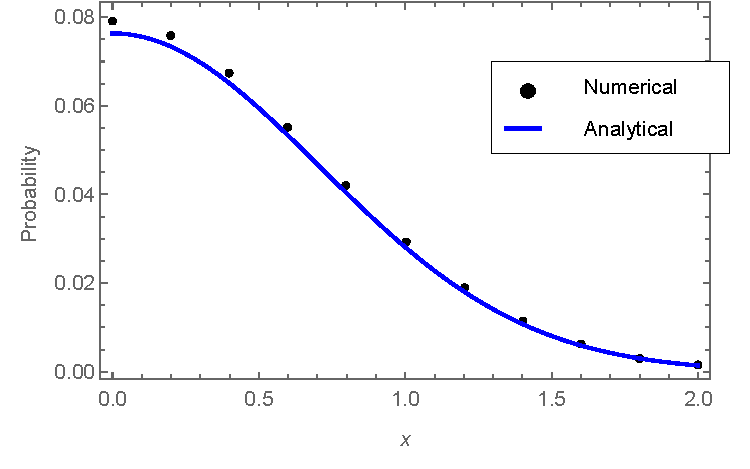
\includegraphics[trim={0 0.7cm 0 0}]{Quantum_Oscillator_Path_Integral.pdf}
	\caption{Plot of $\mel{x}{e^{-Ht}}{x}$ for various values of $x$ calculated using equations \ref{eq:PathIntNum} and \ref{eq:ActionTot}. The blue line represents the analytic solution where $\mel{x}{e^{-H\Delta t}}{x}\approx\abs{\bra{x}\ket{E_0}}^2e^{-E_0\Delta t}$ and $\bra{x}\ket{E_0}=\exp(-x^2/2)/\pi^{1/4}$.}
	\label{fig:QHO}
\end{figure}

\subsection{Monte Carlo Application}
\subsubsection{Manipulation for Monte Carlo}
The above derivation is in regards to the ground state of the system. In systems such as those found in quantum field theory, the ground state is a vacuum and the measurement of observables in excited states is desired. The vacuum expectation value $\expval{x(t_2)x(t_1)}{0}$ can be written as the correlation function
\begin{align}
	\langle x(t_1)x(t_2)\rangle=\frac{\int \mathcal{D}[x(t)]x(t_2)x(t_1)e^{-S[x]}}{\int \mathcal{D}[x(t)]e^{-S[x]}}
	\label{eq:CorFunction}
\end{align}
where $t_i<t_1<t_2<t_f$. Notice that equation \ref{eq:CorFunction} is written in the Heisenberg picture; the operators are time-dependent (in this case the position operators). If we change to the Schr\"odinger picture, this equation can be rewritten keeping in mind the rotation to Euclidean time as
\begin{align}
	\langle x(t_1)x(t_2)\rangle&=\frac{\int\dd{x}\mel{0}{e^{-H(t_f-t_2)}}{x}\mel{x}{e^{-H(t_2-t_1)}}{x}\mel{x}{e^{-H(t_1-t_i)}}{0}}{\int\dd{x}\mel{0}{e^{-H(t_f-t_i)}}{0}}.\\
	\intertext{The numerator can be seen as an interruption on equation \ref{eq:ContPathInt} with the position operator $x$ at $t_1$ and $t_2$. Simplifying, we have}
	&=\frac{\int\dd{x}\mel{0}{e^{-H(t_f-t_2)}xe^{-H(t_2-t_1)}xe^{-H(t_1-t_i)}}{0}}{\int\dd{x}\mel{0}{e^{-H(t_f-t_i)}}{0}}.\\
	\intertext{A further simplification can be made by inserting the the complete set of states $\sum_i\ket{E_i}\bra{E_i}=1$ twice for $i=m,n$ next to the vacuum bra and ket. Letting $T=t_f-t_i$ and $t=t_2-t_1$, this ultimately yields}
	&=\frac{\sum_ne^{-E_nT}\mel{E_n}{xe^{-(H-E_n)t}x}{E_n}}{\sum_ne^{-E_nT}}.
\end{align}
Making the assumption that $T$ is large and $T\gg t$, the first term will dominate due to the exponential and we end up with
\begin{align}
	\langle x(t_1)x(t_2)\rangle=\mel{E_0}{xe^{-(H-E_0)t}x}{E_0}.
\end{align}

For the harmonic oscillator, if a complete set of states is inserted, only the $E_1$ states survive and thus we have
\begin{align}
	\langle x(t_1)x(t_2)\rangle&=\mel{E_0}{x}{E_1}\mel{E_1}{e^{-(H-E_0)t}}{E_1}\mel{E_1}{x}{E_0}\\
	&=\abs{\mel{E_0}{x}{E_1}}^2e^{-(E_1-E_0)t}
\end{align}
where we can now find the difference $E_1-E_0$. There is the unknown transition amplitude matrix element but if we let $G(t)=\langle x(t_1)x(t_2)\rangle$, then
\begin{align}
	E_1-E_0=\frac{1}{a}\log\left[\frac{G(t)}{G(t+a)}\right].
	\label{eq:ExciteE}
\end{align}
The quantity $G(t)$ can be considered as a weighted average from equation \ref{eq:CorFunction} with the weight being the exponential $\exp(-S[x])$. If the probability of the paths being drawn is proportional to this weight and the number of paths is large, then the weighted average can be approximated with an unweighted average. This means that
\begin{align}
	G(t)=\langle x(t_1)x(t_2)\rangle\approx\frac{1}{N}\sum_{n=1}^Nx_n(t_1)x_n(t_2)
	\label{eq:GApprox}
\end{align}

We now have everything needed to write a Metropolis algorithm program to generate an ensemble of paths. The process is analogous to the Ising model but with one exception: the value a site (or, in this case, a time slice) may have is not limited to only either $+1$ or $-1$ (as with the Ising model). Rather, a small random number $\alpha$ is added to the time slice to determine if such a change will be accepted by the Metropolis algorithm. Below are the steps to generate one path:
\begin{enumerate}
\item Choose a site $j$ in path $x$.
\item Add a random number $\alpha\in(-\epsilon,\epsilon)$ to the site $x_j$ so that $x_j\to x_j+\alpha$.
\item Calculate the change in action $\Delta S$ due to the change in $x_j$.
\item If $\Delta S<0$, then change the spin at site $j$.
\item Otherwise assign it a probability $\exp(-\Delta S)$ of changing.
\item Repeat steps 1-5 for every site on the path.
\end{enumerate}
The change in action can be written as
\begin{align}
	\Delta S= \frac{\alpha}{a}\left[(a^2+2)x_j+\left(\frac{\alpha^2}{2}+1\right)\alpha-x_{j+1}-x_{j-1}\right]
\end{align}
and, as with the Ising model, periodic boundary conditions are used, so the modulus operator is used for $x_{j+1}$ and $x_{j-1}$. Figure \ref{fig:PathCode} shows the code that applies the steps above.
\begin{figure}[h]
\begin{lstlisting}
def dS(j, alpha):
    deltaS = (alpha / a) * ((a**2 + 2)*x[j] + (a**2/2 + 1)*alpha
    				 - x[(j + 1) % N] - x[(j - 1) % N])
    return deltaS

def update(x):
    for j in range(N):
        alpha = np.random.uniform(-eps, eps)
        deltaS = dS(j, alpha)        
        if deltaS < 0 or np.random.random() < np.exp(-deltaS):    
            x[j] += alpha
\end{lstlisting}
    \caption{Python code for one configuration of a path split into $N$ slices.}
\label{fig:PathCode}
\end{figure}

A few details must be discussed before making measurements. Firstly, is the starting configuration. An initial configuration should be used that is close to the equilibrium. This allows the program to reach equilibrium quicker. A initial configuration of $x_j=0$ for all $j$ is used in this program. One detail is the value of $\epsilon$. This number determines the maximum at which a site can change and there are pros and cons to having both a large or small $\epsilon$. If $\epsilon$ is small, many changes will be accepted but each successive path will be highly correlated. On the other extreme, successive paths will not be very correlated but changes will rarely be accepted. Therefore an $\epsilon$ is chosen by trial and error and $\epsilon=1.4$ is used in this code. Correlated paths are not desirable because the evolution of the path should be independent of previous values of the path. Therefore, not every path created is kept; for this model, every $N_{cor}$th path is recorded where $N_{\text{cor}}=20$. This number is inversely proportional to the lattice spacing $a$ and goes roughly as $N_{\text{cor}}\propto 1/a^2$. In this model, $a$ is large ($a=1/2$), so the choice of $N_{\text{cor}}$ is appropriate. Lastly, the paths must be thermalized before measurements are taken. In other words, the system must reach an equilibrium before paths are recorded and correlation functions measured. The appropriate number for this can also be measured by trial error. Here, $5N_{\text{cor}}$ paths are thrown away before measurements are taken.

\subsubsection{Measurements}
The quantity $G(t)$ can be measured numerically by using equation \ref{eq:GApprox} since the measurement is a simple product but other correlation functions could be calculated  and used by changing that which is used in the function \texttt{computeG} in figure \ref{fig:ComputeG}. The potential (in this case, that of the harmonic oscillator) can also be changed in the function \texttt{dS} in figure \ref{fig:PathCode}.

The correlation function requires the correlation between each pair of sites on the path to be measured for each path. This is shown in figure \ref{fig:ComputeG}. For this code, 10000 paths are created and, to save computing time, binned into 100 different bins. Binning the paths does not change the statistics of the system, but makes calculations much quicker. Since $G(t)$ measures the correlation of two sites on the path and is the sum of a decreasing and an increasing exponential, we expect to see a curve similar to a hyperbolic cosine due to the periodic boundary conditions. This is seen in figure \ref{fig:CorrFunc}; path sites with a further distance between them are less correlated.
\begin{figure}
\begin{lstlisting}
def computeG(x, n):
    g = 0
    for j in range(N):
        g += x[j] * x[(j + n) % N]
    return g / N

def MCPaths(G):
    for i in range(N_cf):
        for j in range(N_cor):
            update(x)

        for k in range(N):
            G[i][k] = computeG(x, k)
\end{lstlisting}
\caption{Python code for calculating the correlation function $G(t)$ assuming it as an unweighted average. The measurement made on the paths is made only after every \texttt{N\_cor} paths and the \texttt{N} slices of each path in stored in the $i$th element of the array \texttt{G}.}
\label{fig:ComputeG}
\end{figure}

\begin{figure}[h]
	\centering
	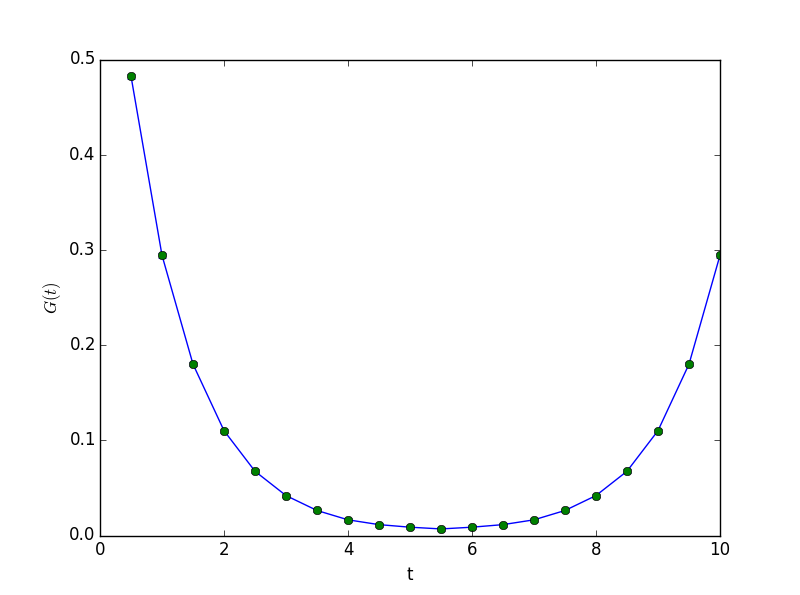
\includegraphics[scale=0.60]{Correlation_Function.png}
	\caption{Measurement of the correlation function for $N=20$ number of sites. The minimum for $G(t)$ is at the maximum distance (or maximum $t$) with periodic boundary conditions (therefore it is found at $N/2$).}
	\label{fig:CorrFunc}
\end{figure}

Using this data, the excitation energy from the ground state can be found by using equation \ref{eq:ExciteE}. This can be rewritten as
\begin{align}
	E_1-E_0=\frac{1}{a}\log\left[\frac{G_n}{G_{n+1}}\right]
	\label{eq:CompExciteE}
	\intertext{where}
	G_n=\frac{1}{N}\sum_{j=1}^Nx_{(j+n)\%N}x_j
\end{align}
and the $\%$ is the modulo operator to take into account the periodic boundary condition. Using equation \ref{eq:CompExciteE}, $N=20$ data points are averaged over 10000 paths. The result is shown in figure \ref{fig:ExciteE}.

The error bars are calculated using the bootstrap method. An ensemble of $N_{cf}$ paths are generated and binned into 100 bins which create 100 new paths that contain the same distribution as the original $N_{cf}$ paths. From the new paths, 100 random paths are selected with replacement which we call the bootstrap paths. The result can contain the same path multiple times as a result. Measurements of $G_n$ and $E_1-E_0$ are completed for the bootstrap paths. The bootstrap method can be calculated many times and distribution of these bootstrap measurements are used to estimate the statistical error of the Monte Carlo measurement of $G_n$ and $E_1-E_0$.

Note that the energy of the quantum harmonic oscillator is $E_n=(n+1/2)\hbar\omega$. So we are expected to see $E_1-E_0=1$ which is what is modeled closely by the data. While there are $N=20$ data points, only 6 are plotted for two reasons. Because of periodic boundary conditions, the data is mirrored for the latter half of the data points. Furthermore, the error grows, which can be seen in figure \ref{fig:ExciteE}, as $t$ gets larger. This is due to randomness of the paths; the plot would asymptotically reach a value of 1 as the number of paths goes to infinity.

\begin{figure}[h]
	\centering
	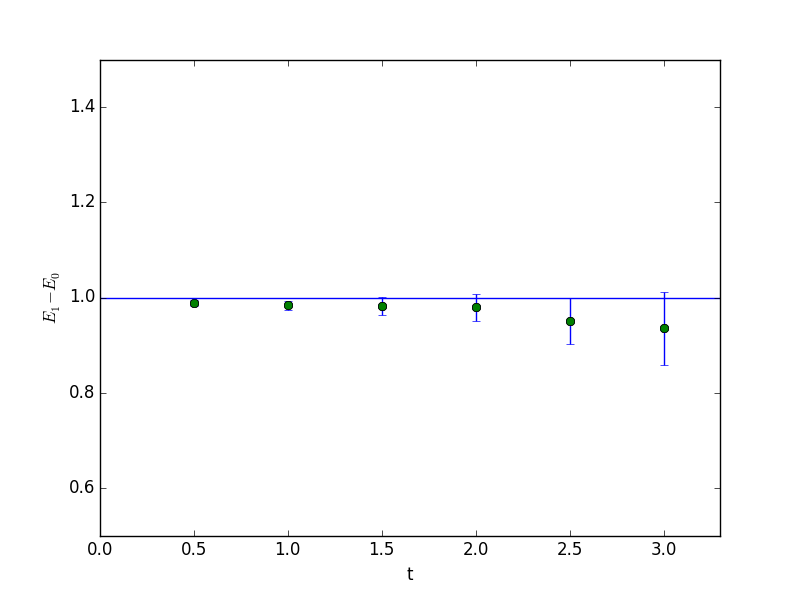
\includegraphics[scale=0.60]{Excitation_Energy.png}
	\caption{Excitation energy of the quantum harmonic oscillator from the ground state. The expected value $E_1-E_0=1$ is represented by the line.}
	\label{fig:ExciteE}
\end{figure}

The harmonic oscillator was used here because of its relatively simple potential $V(x)=x^2/2$ but any potential could be easily applied by using equation \ref{eq:ActionTot} and summing just the $(j-1)$th, $j$th and $(j+1)$th term to calculate the action. Then $\Delta S$ is the difference in action if the $j$th term has some small $\alpha$ added to it. The equation in figure \ref{fig:PathCode} is the simplified equation of $\Delta S$ for the harmonic oscillator. As will be seen in the next section, different measurements can be made relatively easily once the system has been modeled correctly. Here, it was the path integral on a one-dimensional quantum mechanical system. In the next section, it will be the path integral in spacetime for gluons.

\end{document}